\documentclass[9pt]{beamer}

\include{template}
\usetheme[sectionpage=progressbar,block=fill]{metropolis}

\RequirePackage{tikz}
\usetikzlibrary{arrows,positioning,fit,calc,positioning,decorations.pathreplacing}
\usepackage[utf8]{inputenc}
\graphicspath{{images/}{images/theme/}}
\usepackage{appendixnumberbeamer}
\usepackage{tabularx}

\usepackage{amsmath} % assumes amsmath package installed
\usepackage{amssymb}  % assumes amsmath package installed
\usepackage{pifont}% http://ctan.org/pkg/pifont
\newcommand{\cmark}{\ding{51}}%
\newcommand{\xmark}{\ding{55}}%

%\usepackage[numbers]{natbib} %Apa style for citation

%% DONNES UTILES A LA PAGE DE TITRE ET AU PIED DE PAGE...

\title[Multi-modal Visual Localization]{Enhancing Visual-Based Localization by  \\
Learning Appearance of Paired Modalities}
\subtitle{}
\author{Nathan Piasco}
\institute{pLaTINUM project, Saint-Mandé} % ON SE SERT DE INSTITUTE POUR METTER LE LIEUX DE LA CONF
\date{26/03/2018}

\definecolor{IGNVert}{RGB}{148, 192,  22}
\definecolor{IGNGris}{RGB}{112, 119, 122}
\definecolor{IGNRouge}{RGB}{255, 100, 100}
\usepackage{ragged2e}
\newcommand{\norm}[1]{\left\lVert#1\right\rVert}


\defbeamertemplate*{footline}{}{%
  \begin{beamercolorbox}[wd=\textwidth, sep=3ex]{footline}%
	\hspace{1cm}
    
\includegraphics[height=0.6cm]{logo/logo_le2i}
	\hspace{0.1cm}
    
\includegraphics[height=0.6cm]{logo/logo_matis}
    \usebeamerfont{page number in head/foot}%
    \usebeamertemplate*{frame footer}
    \hfill%
	\insertsection
    \hfill%
    \usebeamertemplate*{frame numbering}
  \end{beamercolorbox}%
}

\begin{document}

\begin{frame}[plain,c]
	\titlepage
\end{frame}

\begin{frame}[plain,c]
	\tableofcontents
\end{frame}

\section{Introduction}

\label{sec:intro}

\begin{frame}{Indirect methods for VBL}
	
	Visual Based Localization (\textbf{VBL}) aims to recover the pose or position of a visual input query according to a known reference~\cite{Piasco2017}.
	\vfill	
	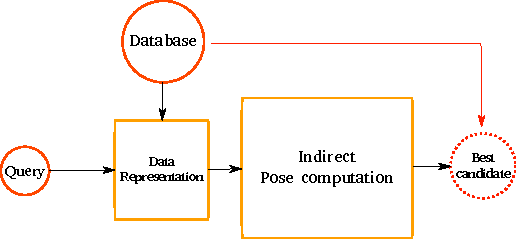
\includegraphics{vect/keys_comp_indirect.pdf}
	
\end{frame}

\begin{frame}{CNN for data representation}
	
	\vfill	
	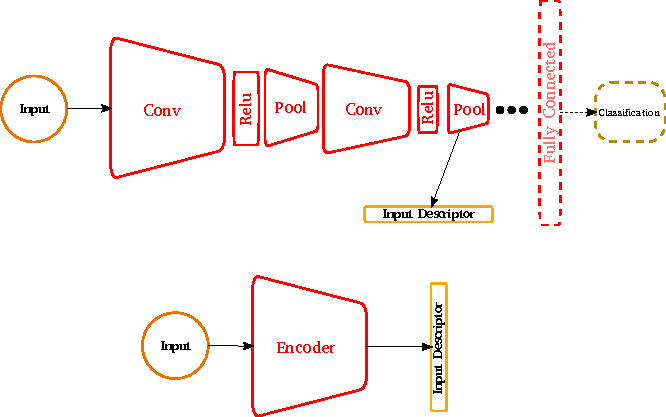
\includegraphics{vect/encodeur.pdf}
	\vfill	
		
\end{frame}


\begin{frame}{Proposed framework}
	\vfill
	\begin{block}{Framework}
		\centering
		\begin{tabular}{c | c}
			\textbf{Training data type} & \textbf{Testing data type} \\
			\hline
			\textbf<2>{RGB + Depth} & \textbf<3>{RGB}  \\
		\end{tabular}
	\end{block}
	\vfill
	\begin{figure}[t]
		\centering
		\uncover<2->{
		\begin{minipage}[b]{0.65\linewidth}
			\centering
			{\footnotesize \textbf{Multi-modal} training dataset}	
	
			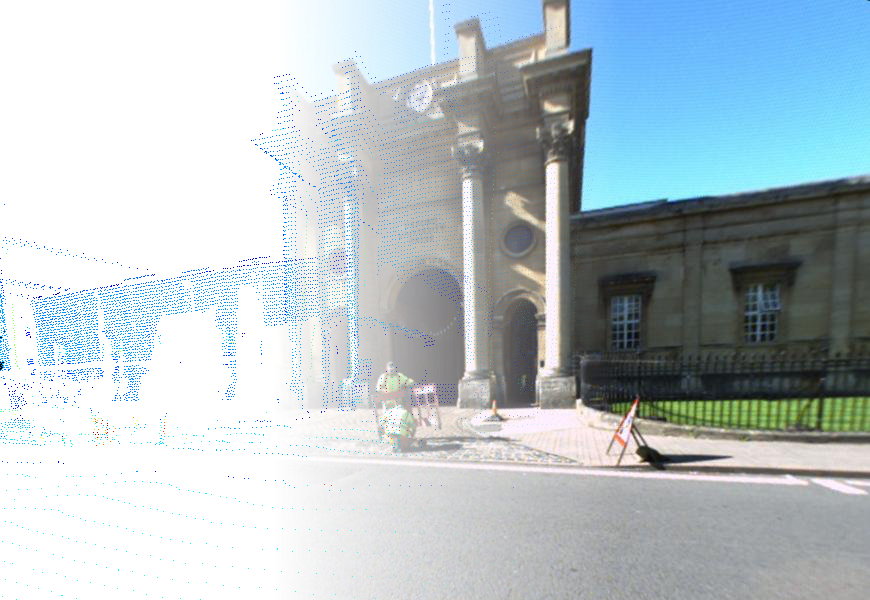
\includegraphics[width=0.51\linewidth]{images/intro_fig/mod0.png}
			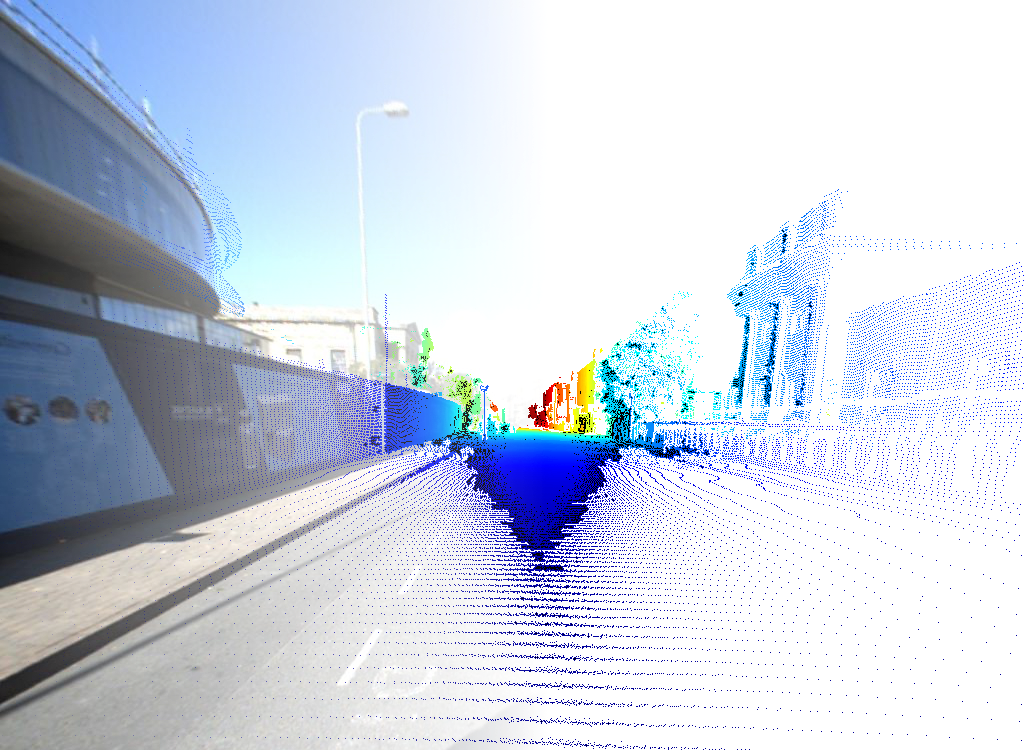
\includegraphics[width=0.47\linewidth]{images/intro_fig/mod1.png}
		\end{minipage}
		}
		\uncover<3>{
		\begin{minipage}[b]{0.32\linewidth}
			\centering
			{\footnotesize \textbf{Single modality} data at test time}
	
			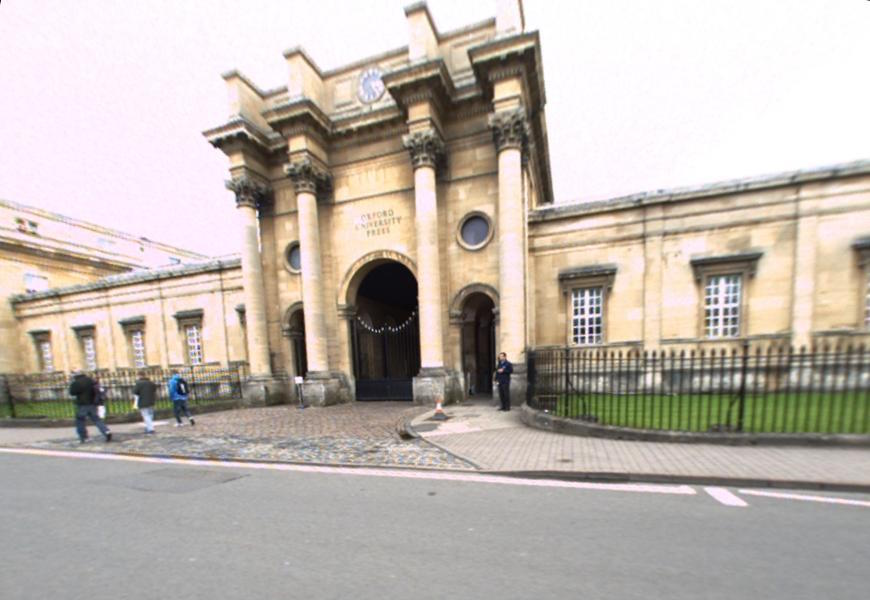
\includegraphics[width=0.85\linewidth]{images/intro_fig/q.jpg}
		\end{minipage}
		}
	\end{figure}
\end{frame}

\section{Related work}

\label{sec:related_work}

\begin{frame}{Feature from CNN}

	\vfill
	\begin{figure}
		\centering
		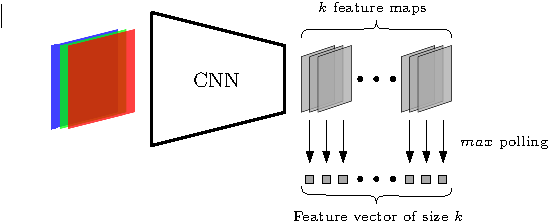
\includegraphics[width=\linewidth, trim = 1cm 0 0 0]{vect/MAC.pdf}			
	\end{figure}

	\vfill
	
	More complex aggregation methods exist: NetVLAD~\cite{Arandjelovic2017}, RMAC...
\end{frame}

\begin{frame}{Learning an image descriptor}

	\begin{minipage}{0.48\linewidth}
		\vfill
		\begin{figure}
			\centering
			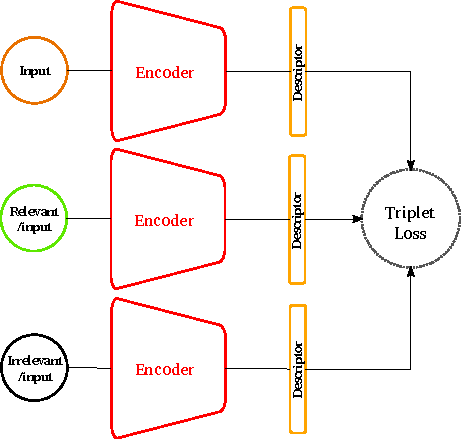
\includegraphics[width=\linewidth]{vect/encoder_training.pdf}			
		\end{figure}
		\vfill
	\end{minipage}
	\begin{minipage}{0.48\linewidth}
		\begin{multline}
			\label{eq:triplet_loss}
			Loss_{triplet} = min\left( \norm{f(q) - f(q^+)}^2 - \right. \\
			\left. \norm{f(q) - f(q^-)}^2 + \lambda, 0\right),
		\end{multline}
		\vfill
		\begin{align*}
		with 
		\begin{cases}
				f(x) = \textnormal{descriptor of image $x$ } \\
				\lambda = \textnormal{triplet loss margin} \\
				q = \textnormal{query image} \\
				q^+ = \textnormal{positif example} \\
				q^- = \textnormal{negatif example} \\
		\end{cases}
		\end{align*}
	\end{minipage}
	
\end{frame}


\begin{frame}{Learning with side modality}
	\vfill
	\begin{figure}
			\centering
			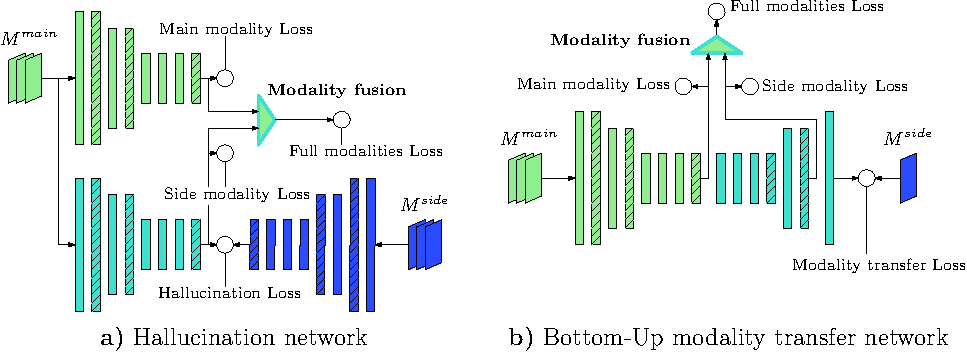
\includegraphics[width=0.48\linewidth, clip=true, trim = 0 0.5cm 8cm 0]{vect/training.pdf}			
			\uncover<2>{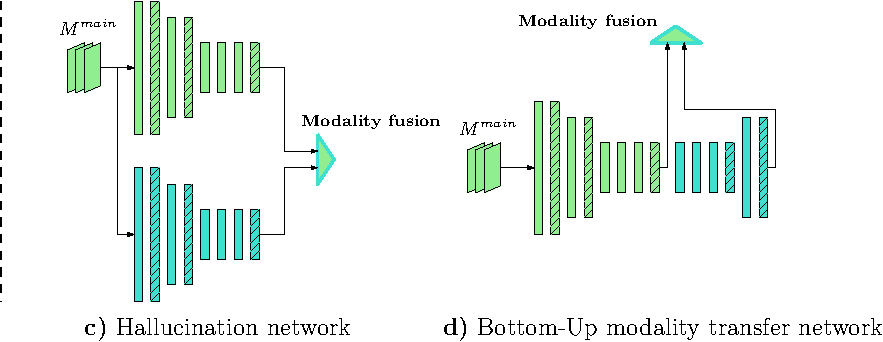
\includegraphics[width=0.48\linewidth, clip=true, trim = 0 0.5cm 7.2cm 0]{vect/testing.pdf}}
		\end{figure}
	\vfill
	Hallucination architecture from~\cite{Hoffman2016}
	\vfill
\end{frame}

\section{Learning side information with modality transfer}

\label{subsec:modality}

\begin{frame}{Proposed architecture}
	\vfill
	\begin{figure}
			\centering
			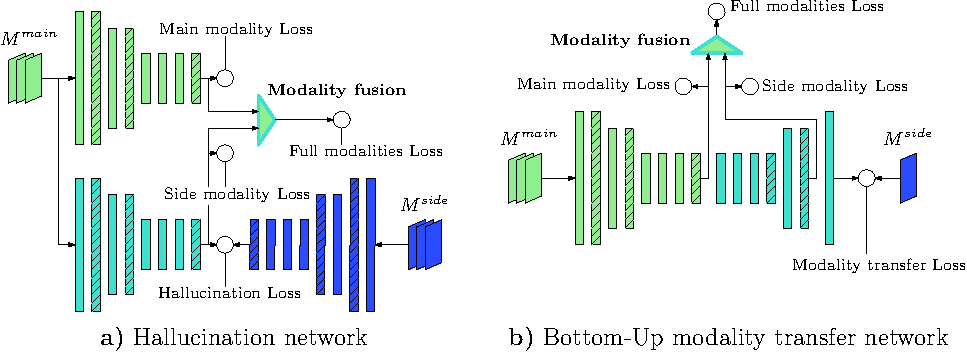
\includegraphics[width=0.48\linewidth, clip=true, trim = 8cm 0.5cm 0 0]{vect/training.pdf} \hfill
			\uncover<2>{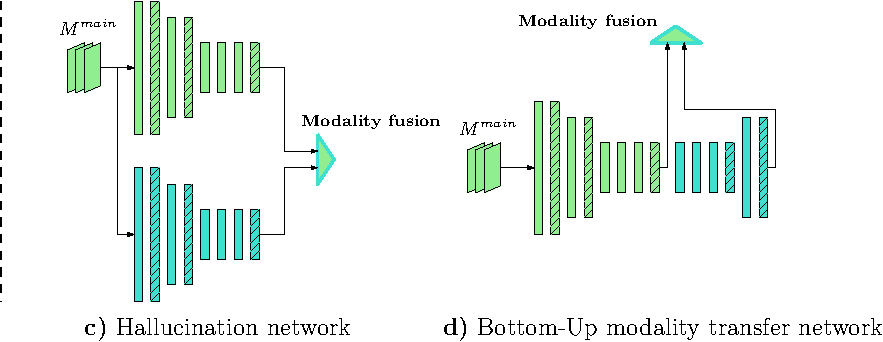
\includegraphics[width=0.48\linewidth, clip=true, trim = 7.6cm 0.5cm 0 0]{vect/testing.pdf}}
		\end{figure}
	\vfill
	The proposed architecture inspired by auto-encoder networks.
	\vfill
\end{frame}

\begin{frame}{Optimization}
	\begin{equation}
			Loss_{transfer} = \norm{\widetilde{M}(M^{main}) - M^{side}}^2,
	\end{equation}
	
	where $\widetilde{M}(x)$ denotes the output of the decoder part of the network regarding input $x$.
	
	\uncover<2->{	
	Final loss:
	\begin{multline}
			Loss = Loss_{triplet}^{main}*\sigma_{main} + Loss_{triplet}^{side}*\sigma_{side} \\
			+ Loss_{triplet}^{full}*\sigma_{full} + Loss_{transfer}*\sigma_{transfer}.
	\end{multline}
	}
	
	\uncover<3>{
	Diversification loss:
	\begin{equation}
		\label{eq:div_loss}
		Loss_{div} = min\left( Loss_{triplet}^{full} - Loss_{triplet}^{main} + \lambda_{div} , 0\right),
	\end{equation}
	where $\lambda_{div}$ is a scalar value that acts as a margin to ensure $Loss_{triplet}^{full}$ is always smaller than $Loss_{triplet}^{main}$.
	}
	
\end{frame}

\begin{frame}{Advantages over hallucination}
	Advantages of our bottom-up transfer approach (\textbf{BU-TF}) over hallucination network are threefold: 
	\begin{itemize}
		\item<2-> No need of pretraining on side modality
		\item<3-> Method by nature lighter: $29k$ parameters vs. $41k$ parameters for networks built upon Alexnet architecture
		\item<4> No need to transform modality into 3-channels data
	\end{itemize}
	

\end{frame}
\section{Experiments}
\begin{frame}{Robotcar dataset}
	\begin{figure}[t]
		\centering
		
		\only<1>{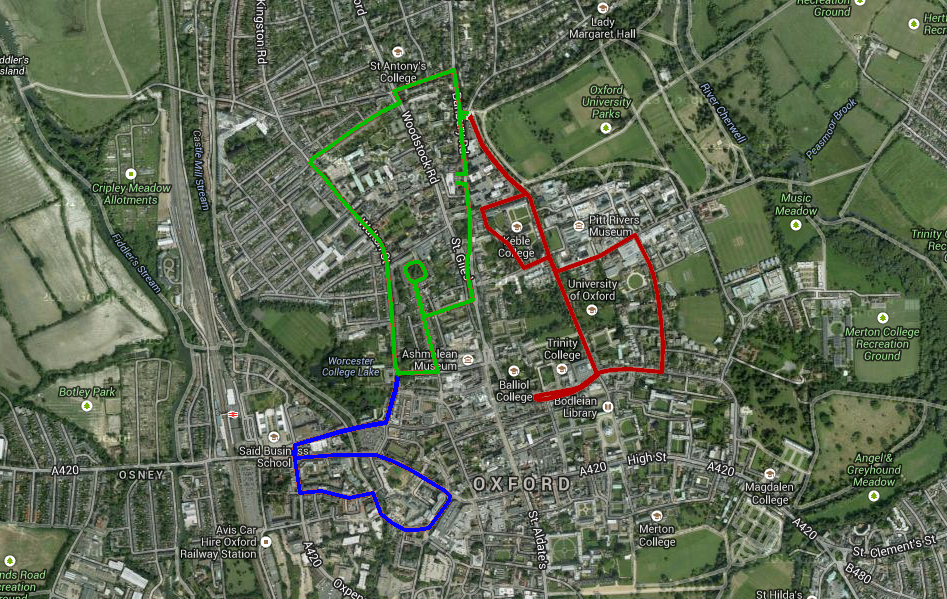
\includegraphics[width=0.8\linewidth]{images/map/map.png}  }
		\only<2>{
		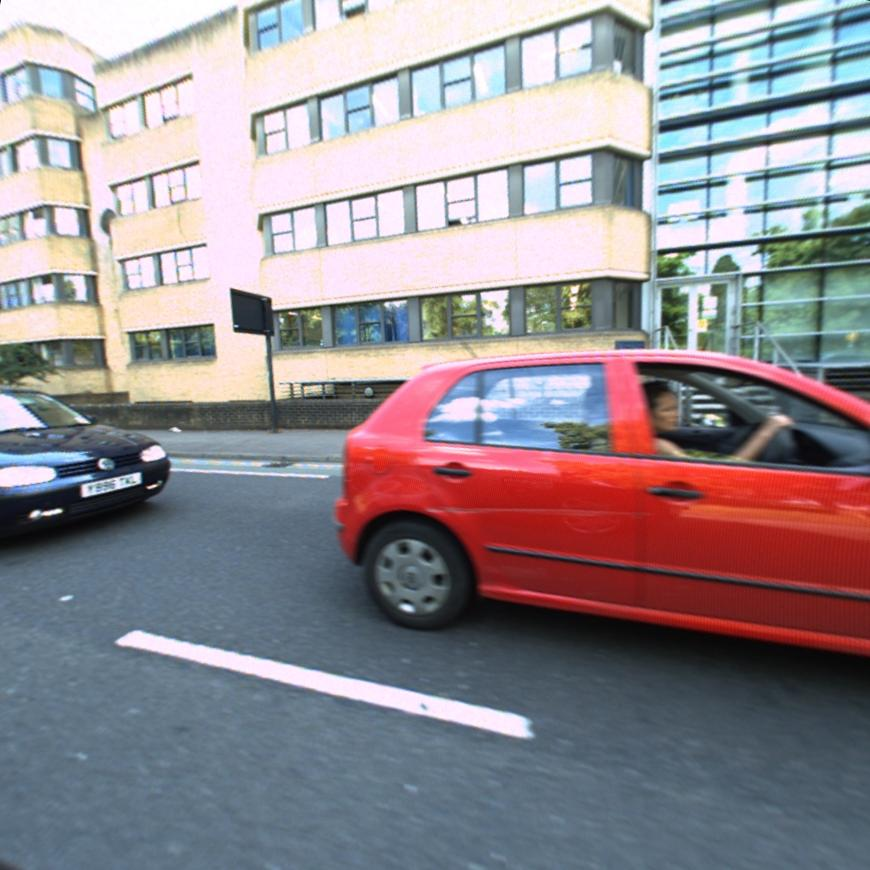
\includegraphics[width=0.19\linewidth]{images/ex_query/query0.jpg}\hfill
		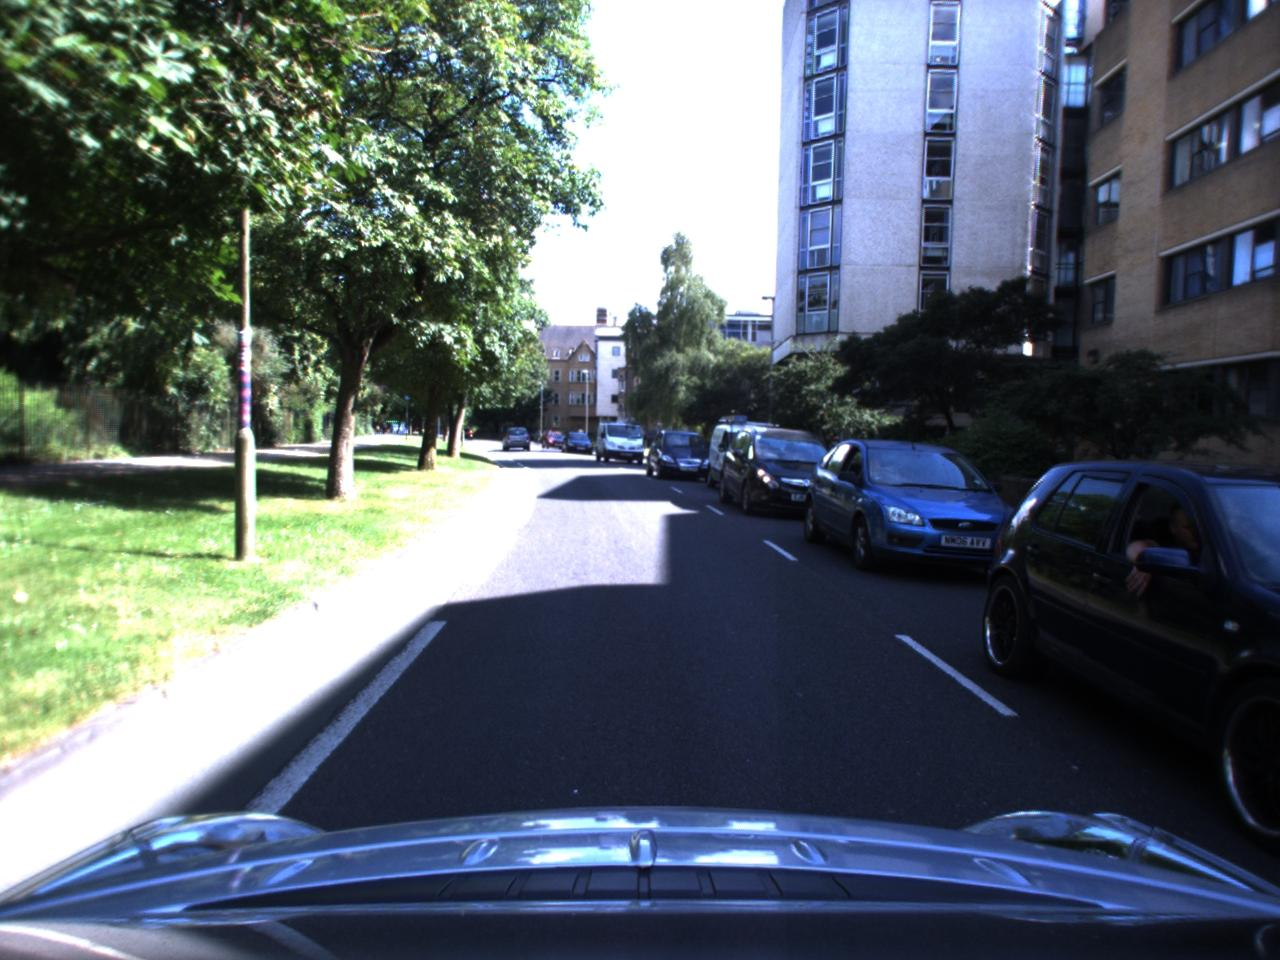
\includegraphics[width=0.23\linewidth]{images/ex_query/query1.jpg}\hfill
		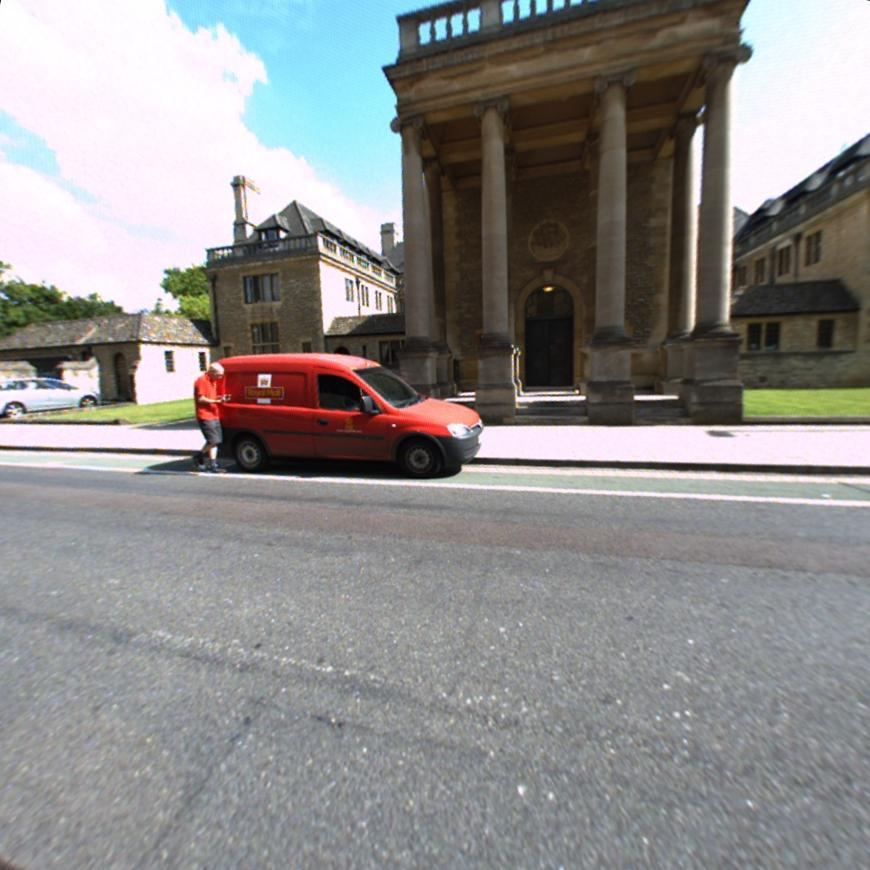
\includegraphics[width=0.19\linewidth]{images/ex_query/query2.jpg}\hfill
		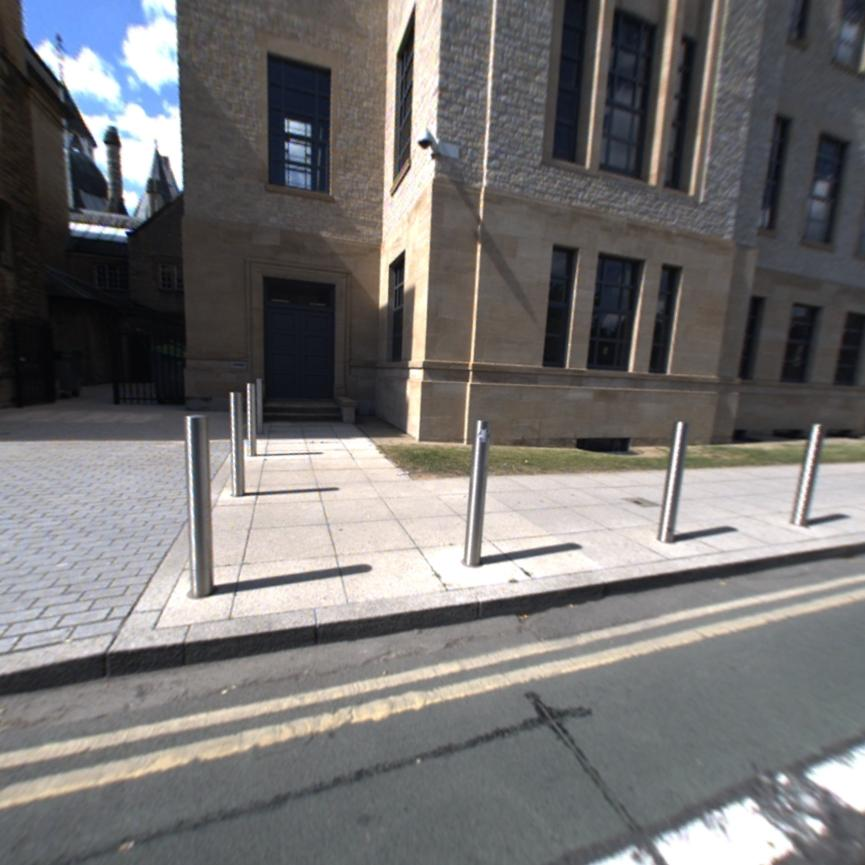
\includegraphics[width=0.19\linewidth]{images/ex_query/query3.jpg}\hfill
		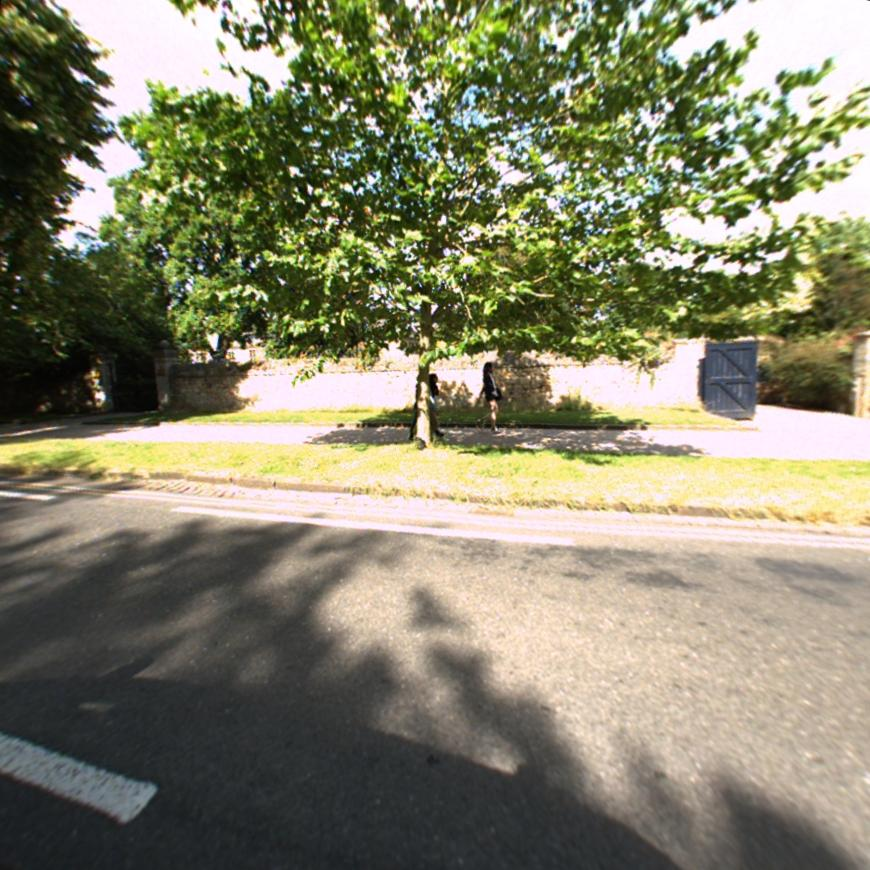
\includegraphics[width=0.19\linewidth]{images/ex_query/query4.jpg}
			
		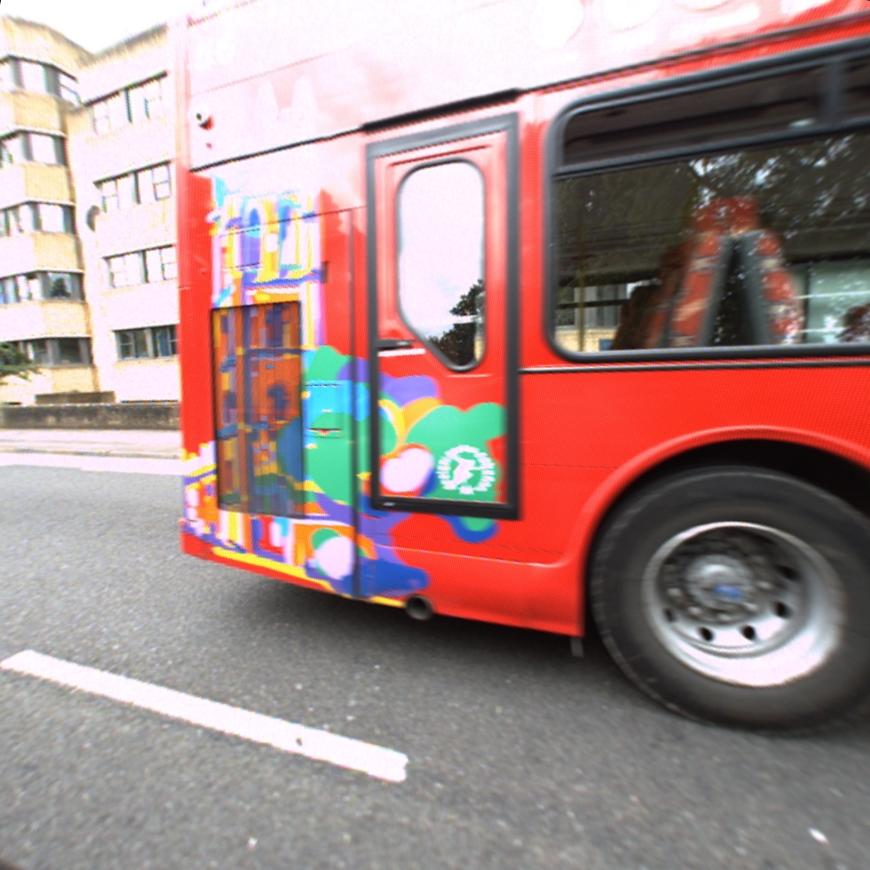
\includegraphics[width=0.19\linewidth]{images/ex_query/dataset0.jpg}\hfill
		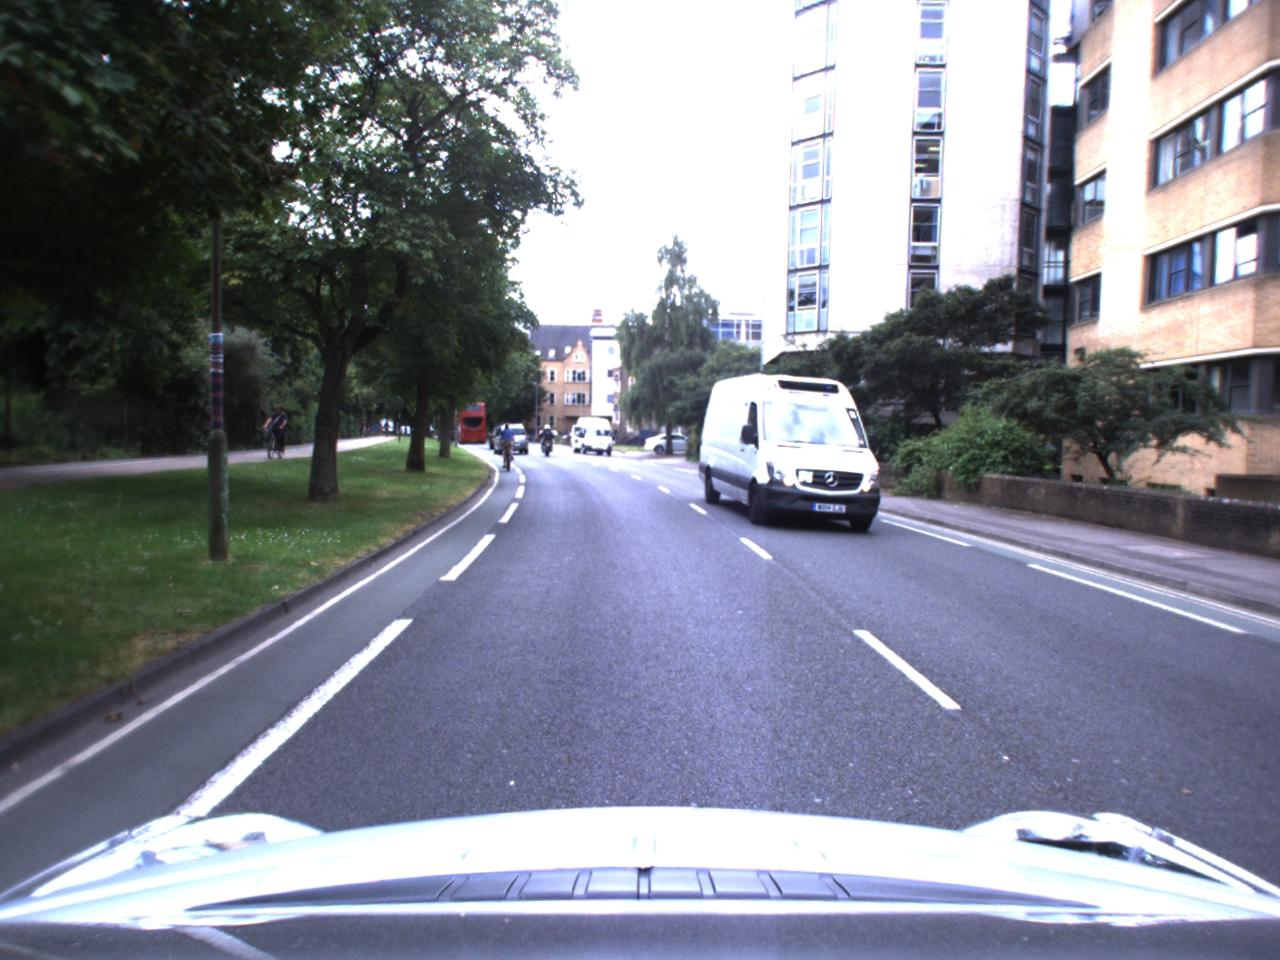
\includegraphics[width=0.23\linewidth]{images/ex_query/dataset1.jpg}\hfill
		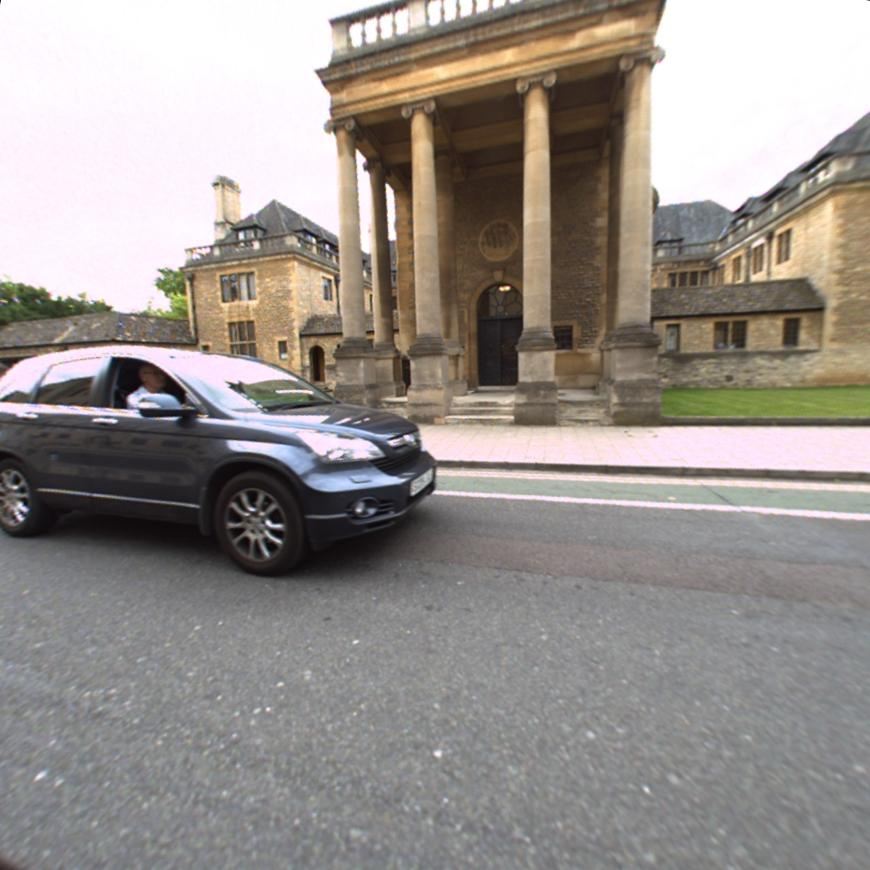
\includegraphics[width=0.19\linewidth]{images/ex_query/dataset2.jpg}\hfill
		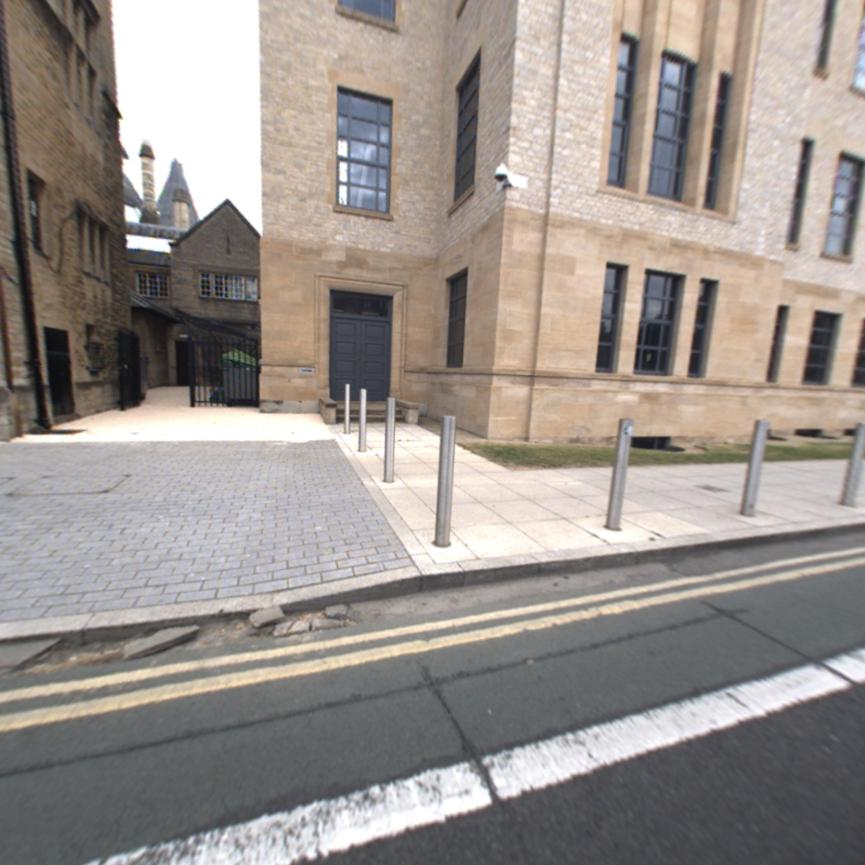
\includegraphics[width=0.19\linewidth]{images/ex_query/dataset3.jpg}\hfill
		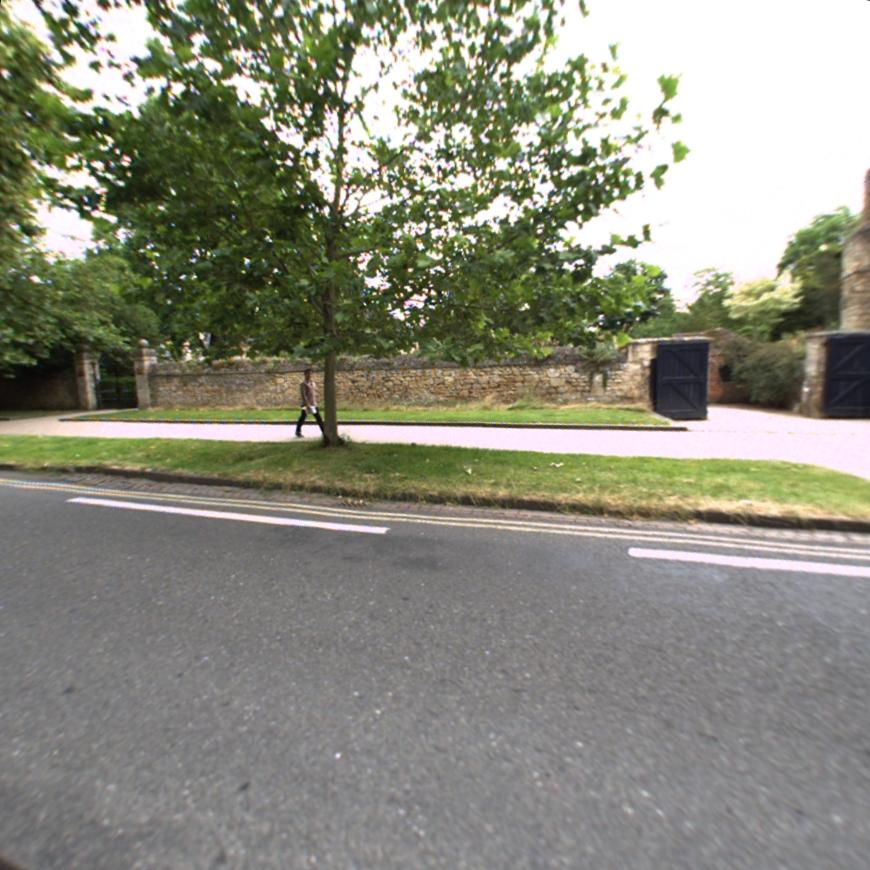
\includegraphics[width=0.19\linewidth]{images/ex_query/dataset4.jpg}
		}
	\end{figure}
	
	\only<1>{Dataset training (green), validation (blue) and testing (red) areas.}
	\only<2>{Examples of queries with corresponding dataset candidates of the testing set.}
\end{frame}

\begin{frame}{Building dense modality map}
	\begin{figure}[t]
			\newcolumntype{Y}{>{\centering\arraybackslash}X}
			\centering
			\begin{footnotesize}
			\begin{tabularx}{\linewidth}{Y Y Y}
				\textbf{Image}	  & \textbf{Points cloud} 			& \uncover<2>{\textbf{Dense depth map}}
			\end{tabularx}
			\end{footnotesize}
			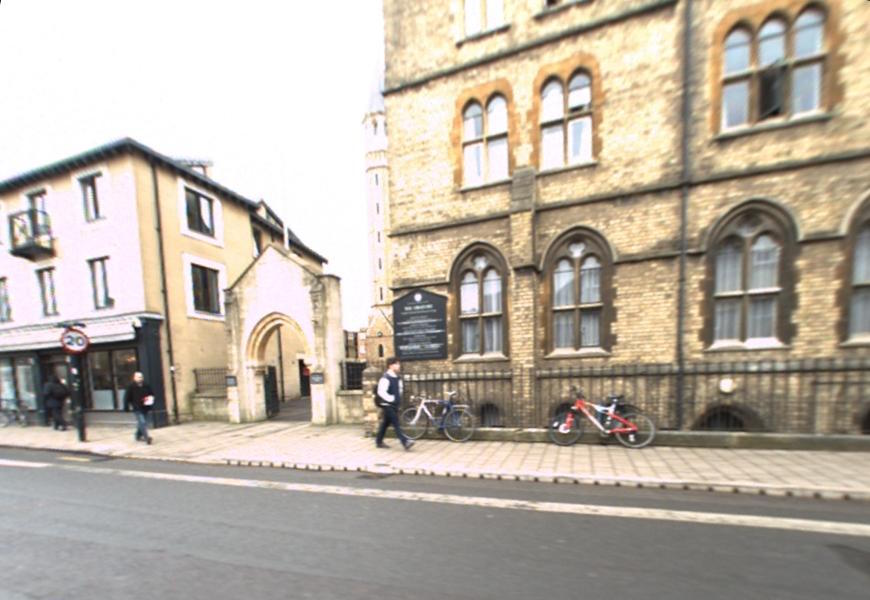
\includegraphics[width=0.33\linewidth]{images/dense_map_creation/image0.jpg}\hfill
			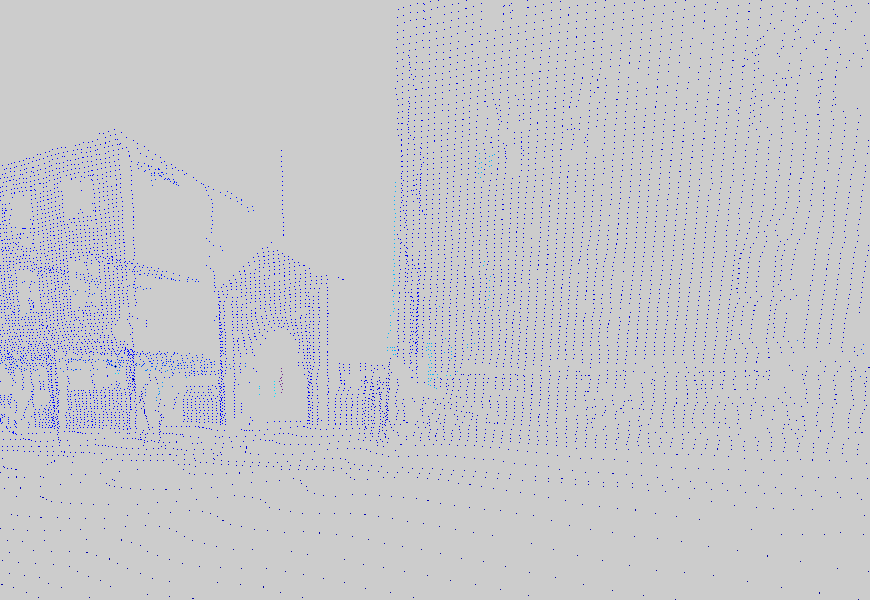
\includegraphics[width=0.33\linewidth]{images/dense_map_creation/sparsedepth0.png}\hfill
			\uncover<2>{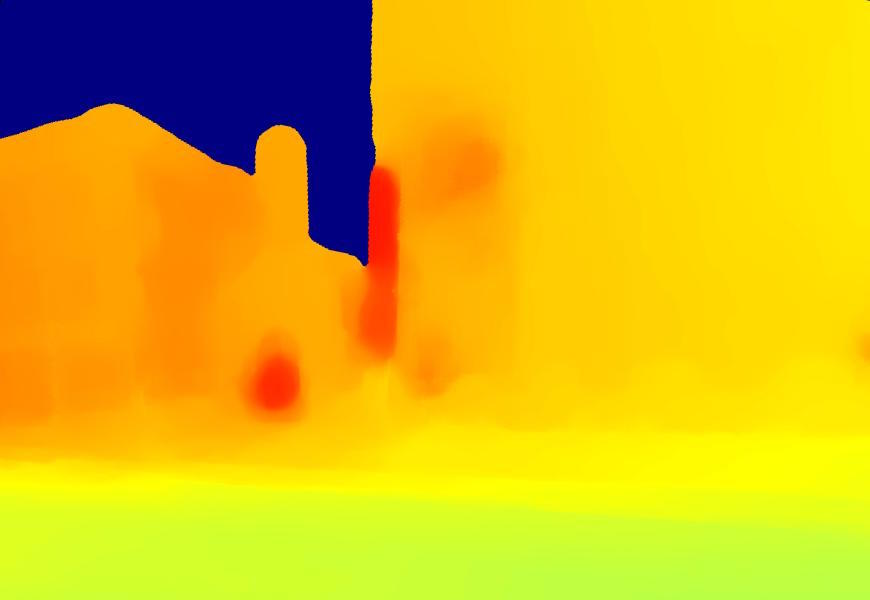
\includegraphics[width=0.33\linewidth]{images/dense_map_creation/densedepth0.jpg}}\hfill
			
			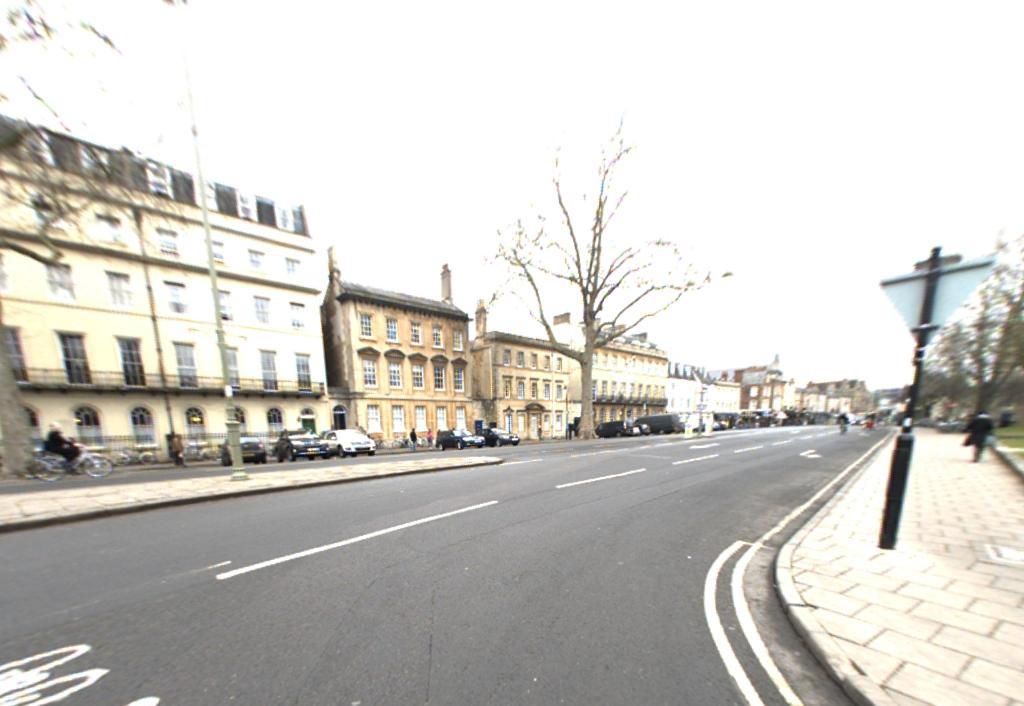
\includegraphics[width=0.33\linewidth]{images/dense_map_creation/image1.jpg}\hfill
			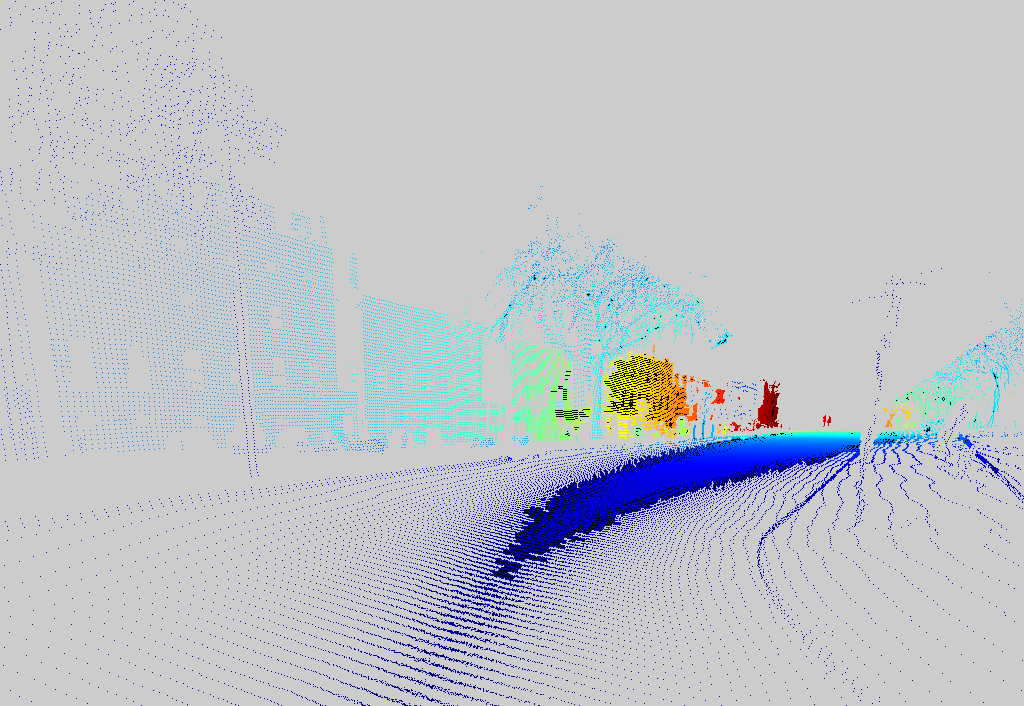
\includegraphics[width=0.33\linewidth]{images/dense_map_creation/sparsedepth1.png}\hfill
			\uncover<2>{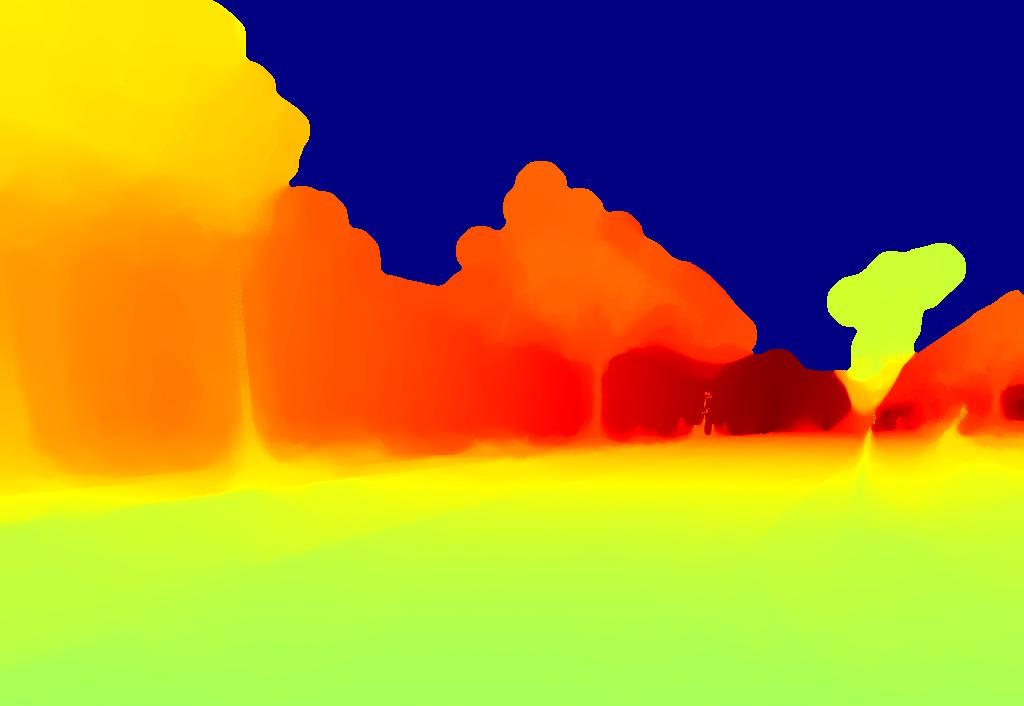
\includegraphics[width=0.33\linewidth]{images/dense_map_creation/densedepth1.jpg}}\hfill
	\end{figure}
	
	We use the algorithm proposed in~\cite{Bevilacqua2017} to create a dense modality map from an image and the associated point cloud.
\end{frame}

\begin{frame}{Results}
	\begin{figure}[t]
		\centering
		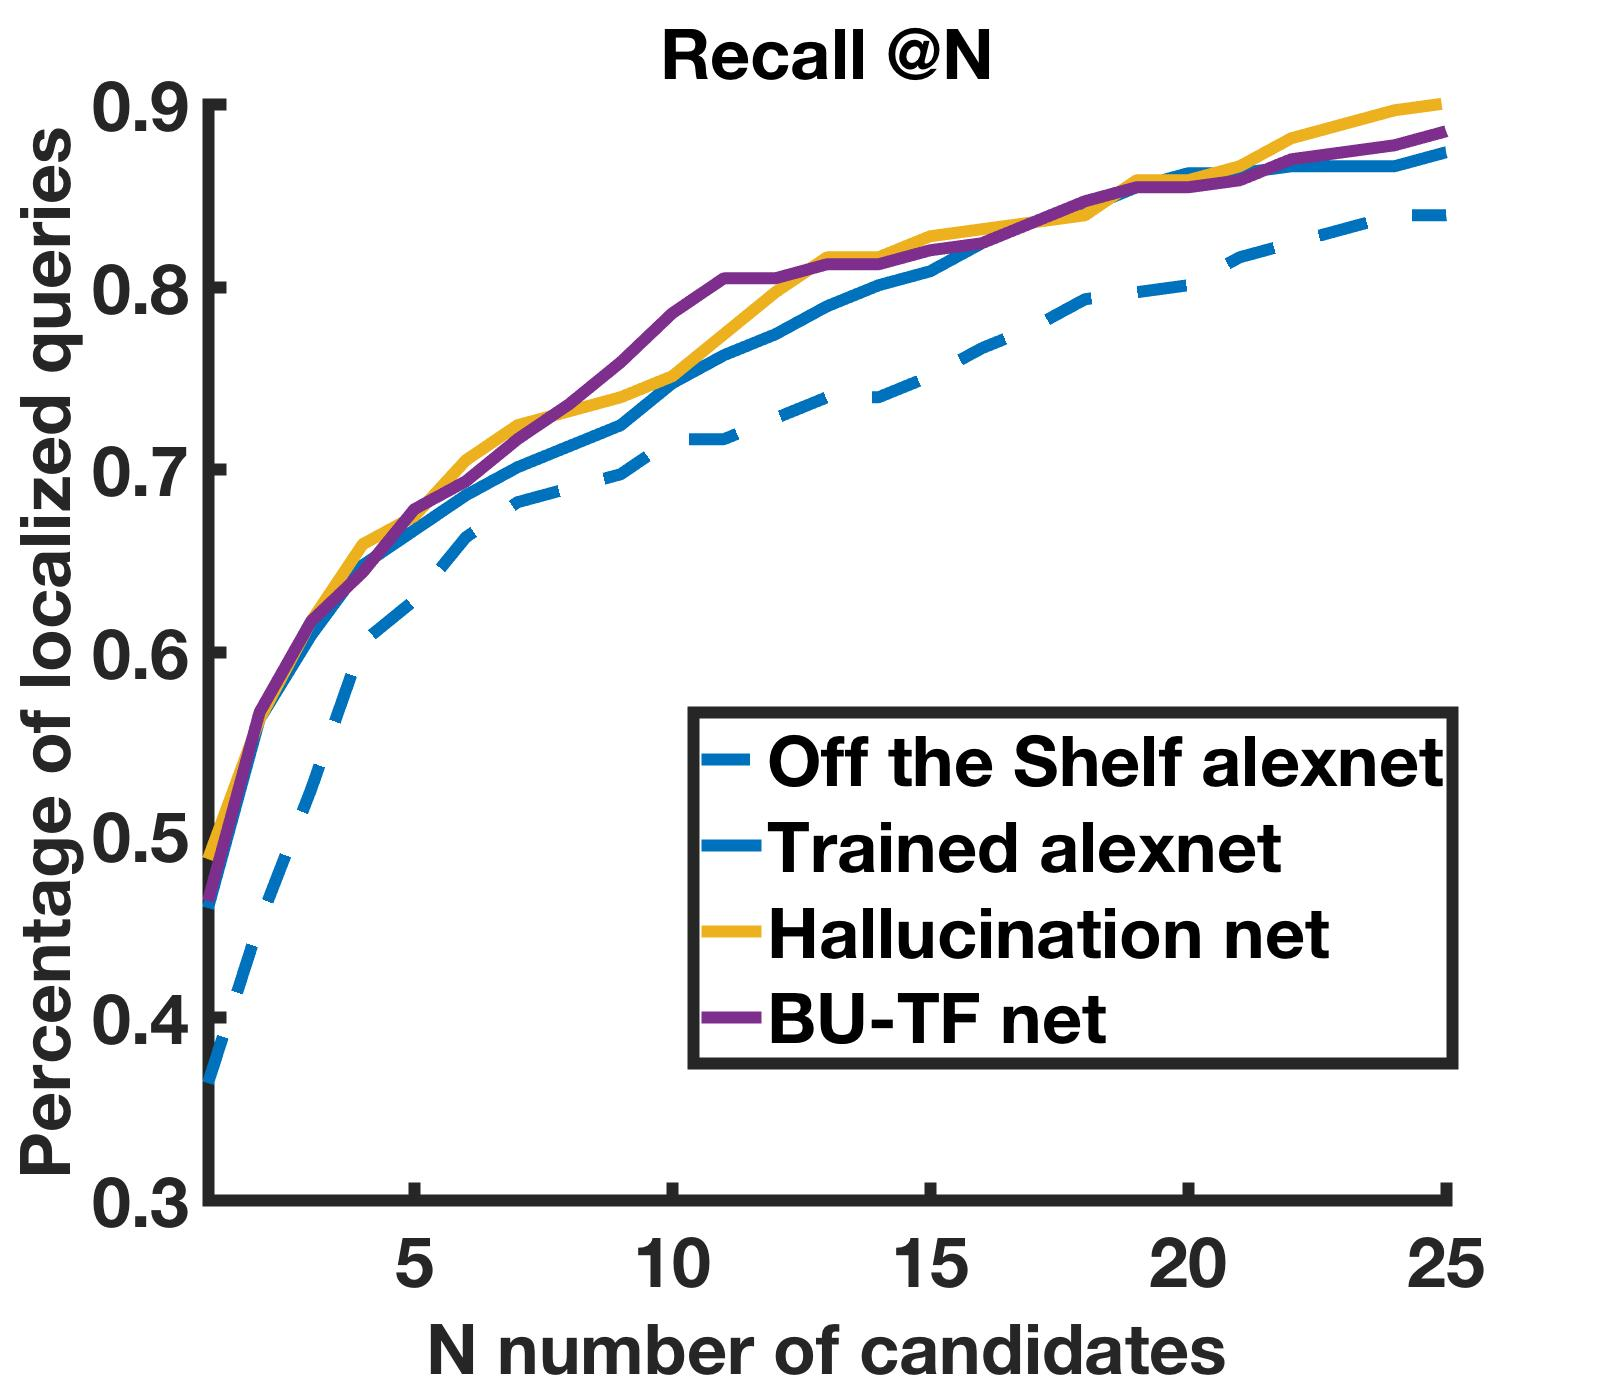
\includegraphics[width=0.499\linewidth]{images/global_res/recall.jpg}\hfill
		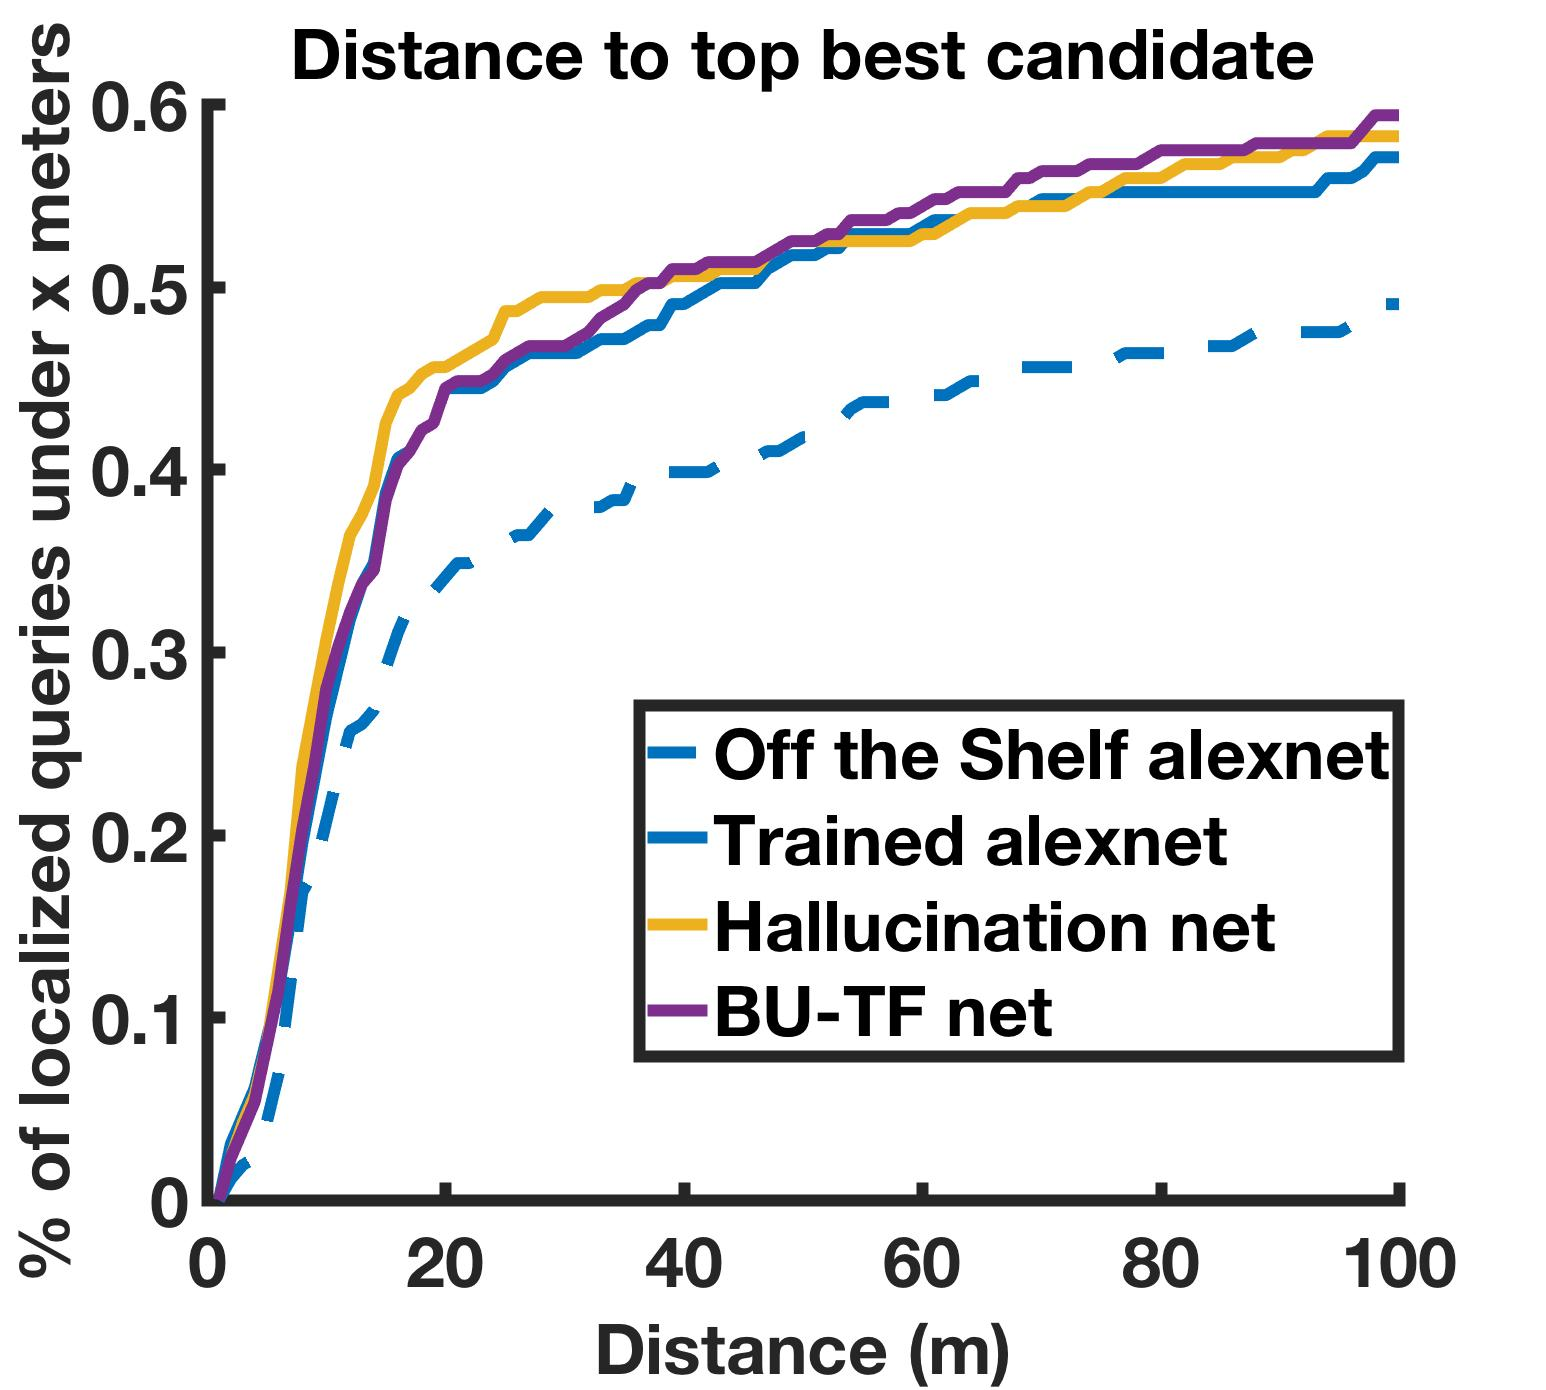
\includegraphics[width=0.499\linewidth]{images/global_res/dist.jpg}			
	\end{figure}	
	Off-the-shelf: network only trained on ImageNet, no fine-tuning for this specific task and on these specific data.
\end{frame}

\begin{frame}{Results - Diversification loss}
	\begin{figure}[t]
		\centering
		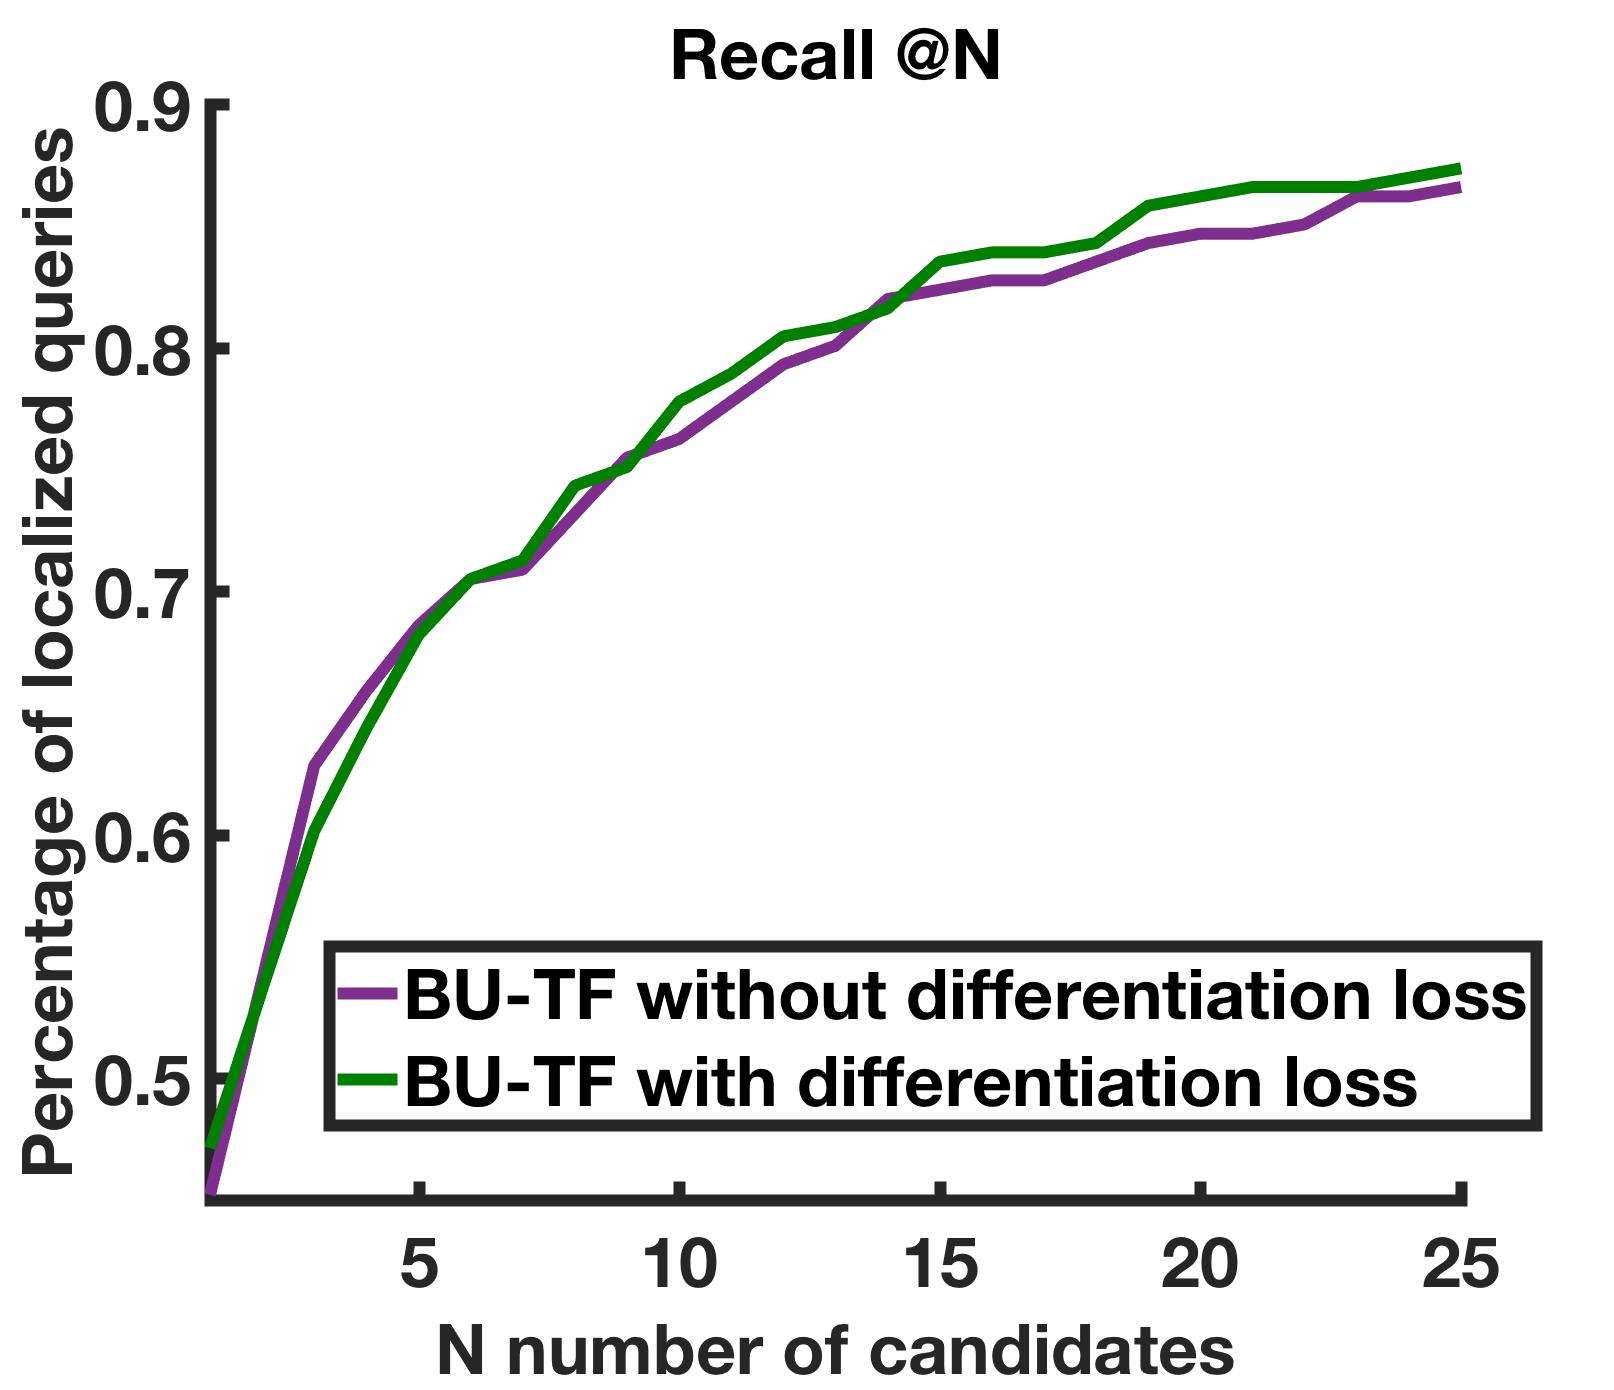
\includegraphics[width=0.499\linewidth]{images/diffloss_res/recall.jpg}\hfill
		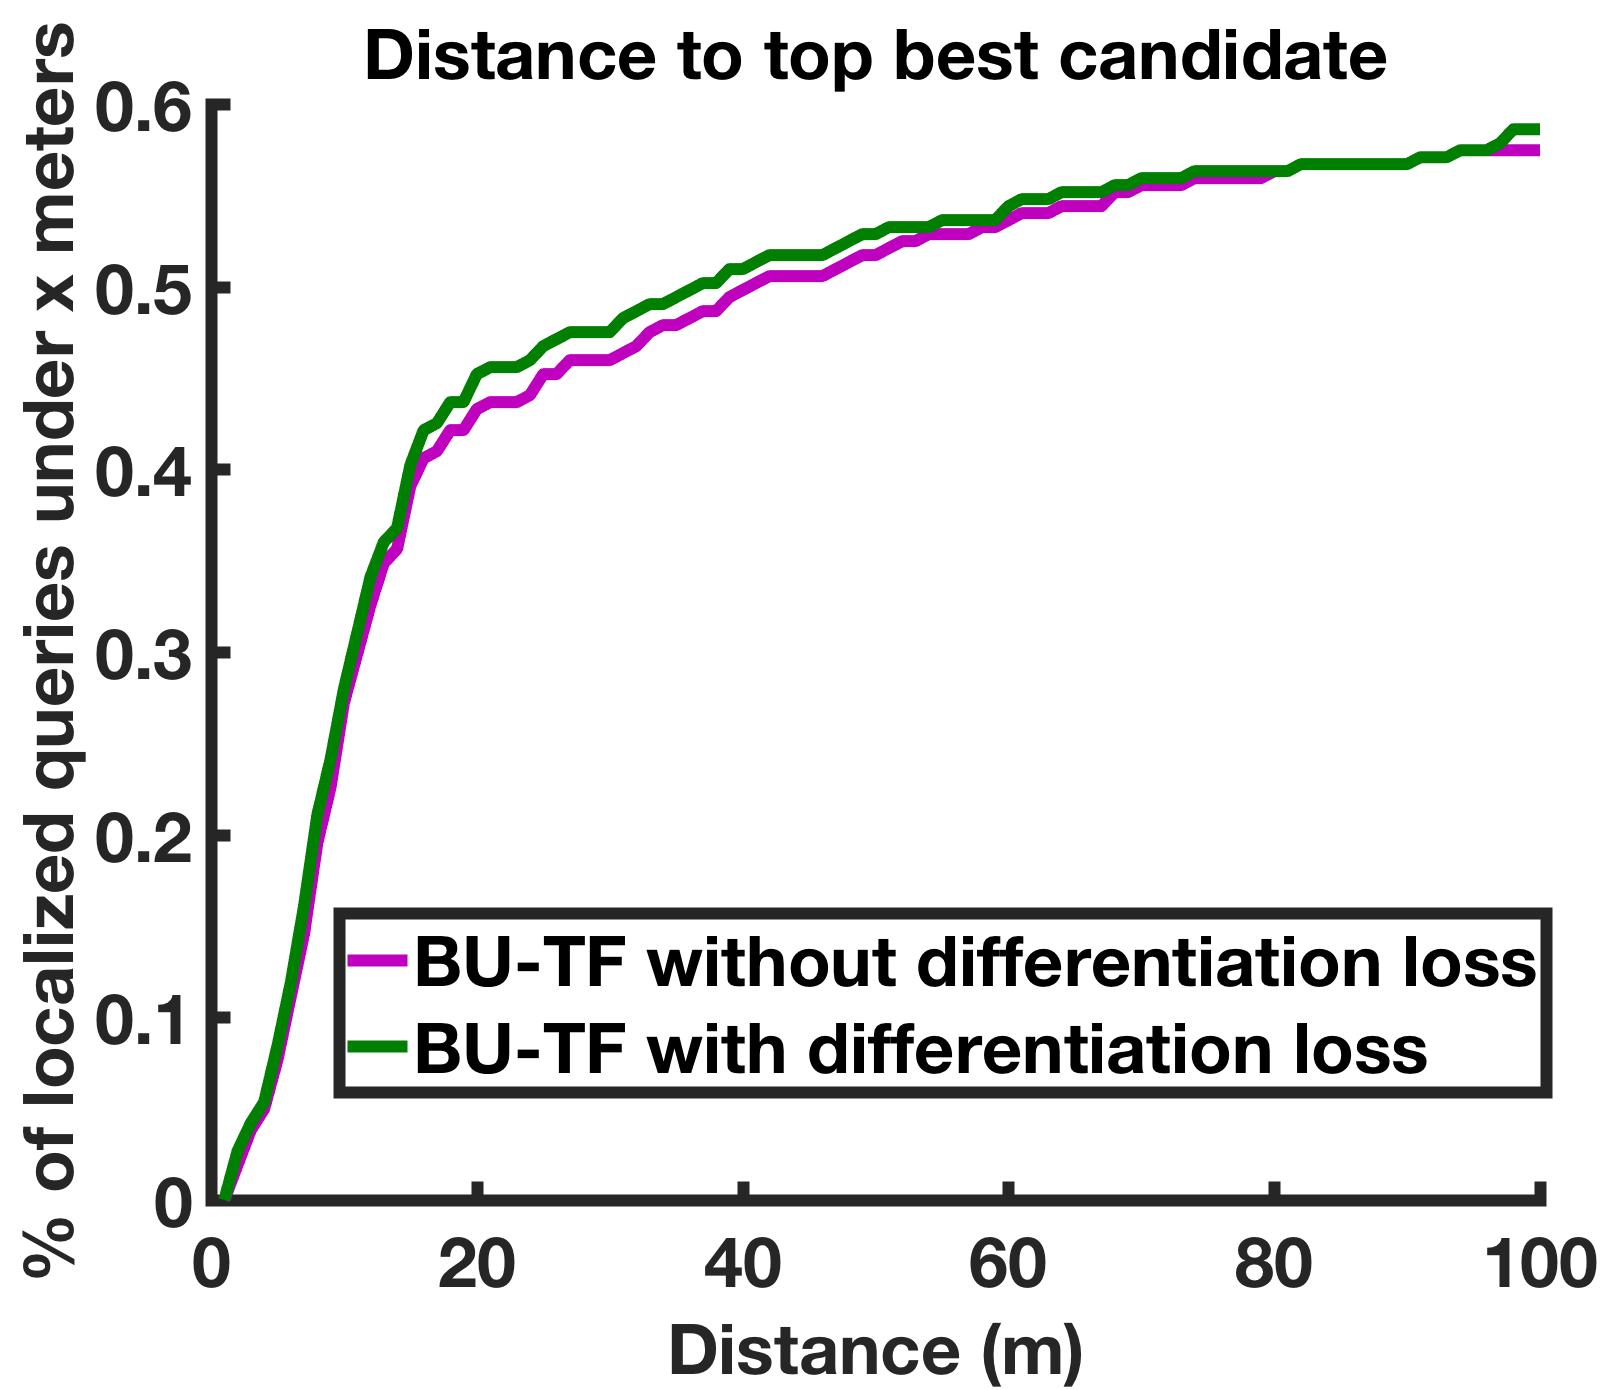
\includegraphics[width=0.499\linewidth]{images/diffloss_res/dist.jpg}			
	\end{figure}	
\end{frame}

\begin{frame}{Smarter modality fusion}
	\begin{figure}
		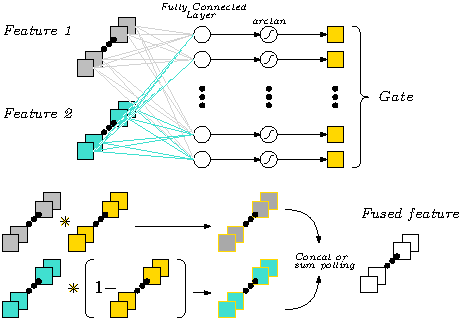
\includegraphics[width=0.8\linewidth]{vect/GatedFuse.pdf}\hfill
	\end{figure}
	
	Inspired from GRU (Gated Recurrent Unit) architecture.
\end{frame}

\begin{frame}{Result - Modality fusion}
	\begin{figure}[t]
		\centering
		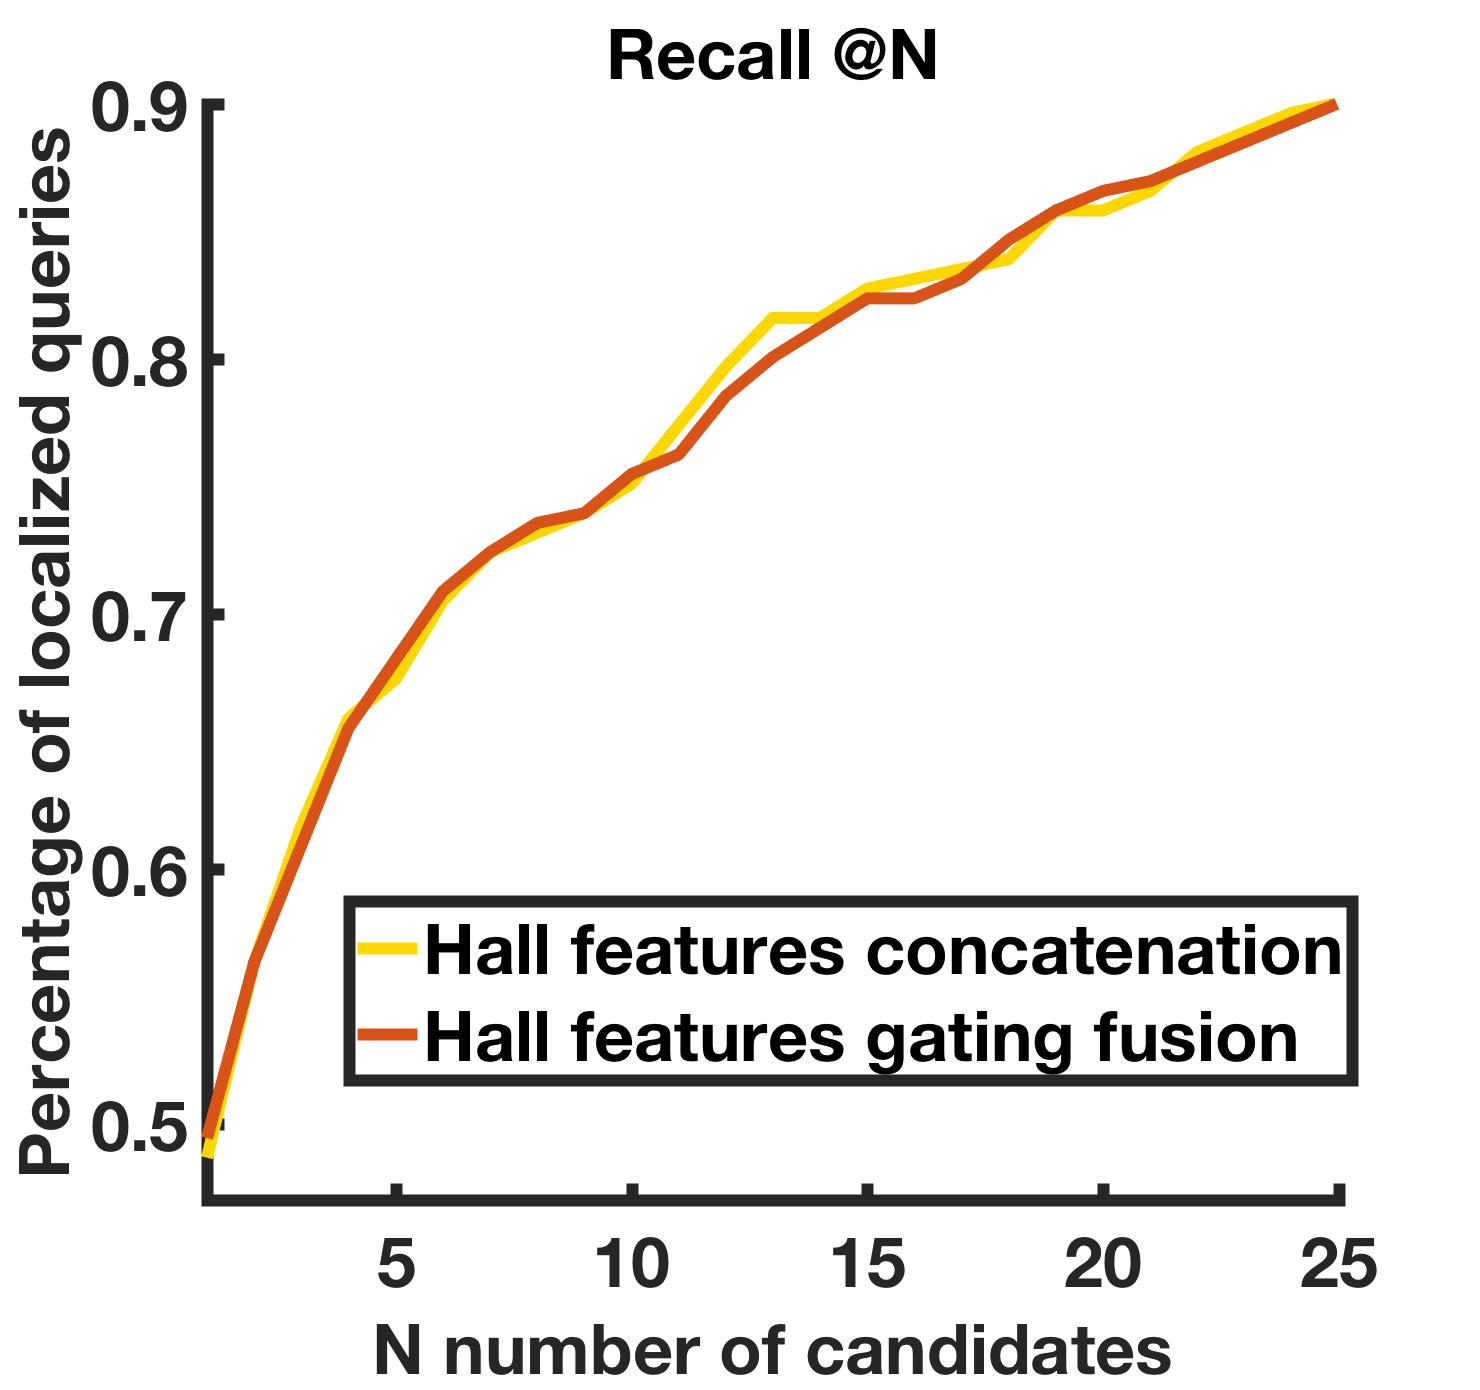
\includegraphics[width=0.499\linewidth]{images/gate_res/recall.jpg}\hfill
		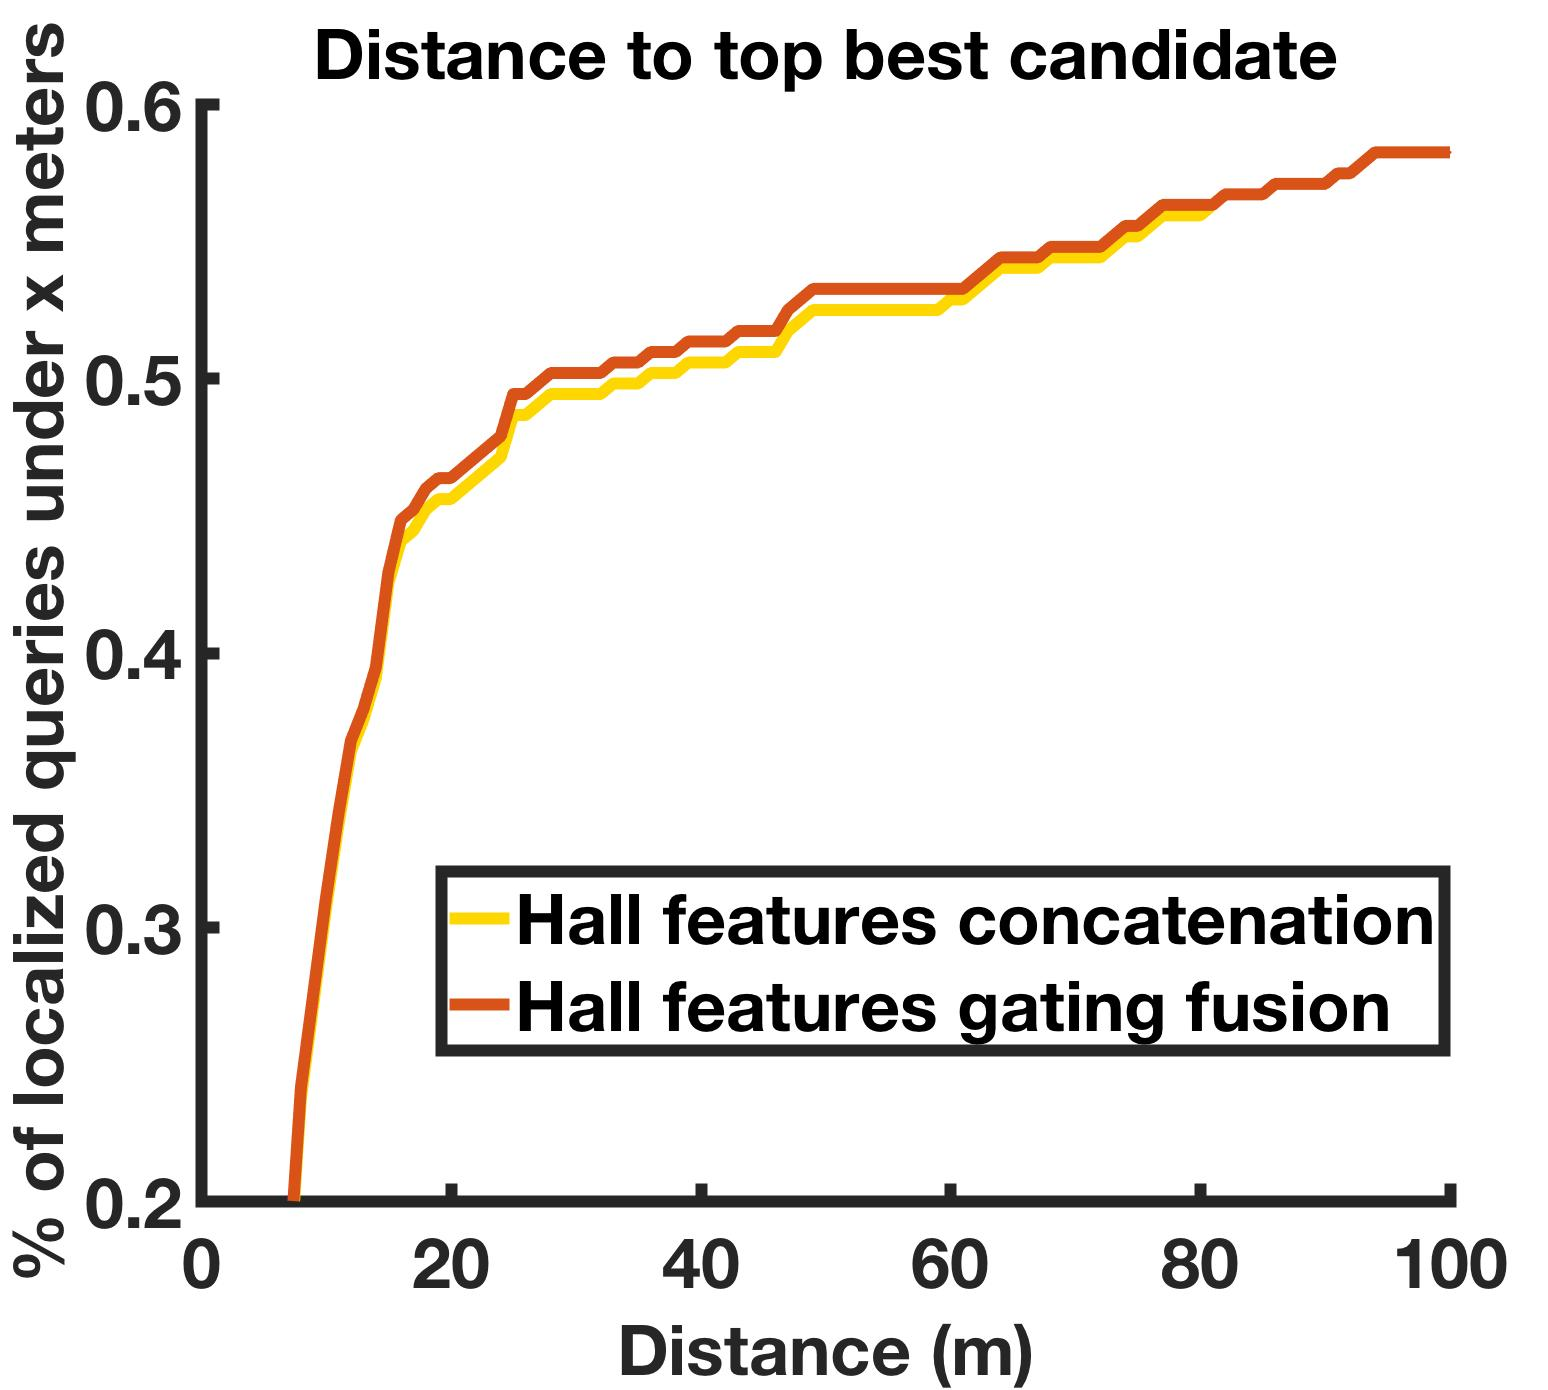
\includegraphics[width=0.499\linewidth]{images/gate_res/dist.jpg}			
	\end{figure}	
\end{frame}
\section{Conclusion}

\label{subsec:conlusion}

\begin{frame}{Conclusion}
	\vfill
	New method for learning with modality side modality have been presented. BU-TF is more efficient than hallucination as it needs less training time have less parameters while producing comparable results.
	\vfill
	\uncover<2->
	{
		The presented method has to be tested:
		\begin{itemize}
			\item<3-> on over modalities
			\item<4-> with other aggregation scheme
			\item<5-> on other visual localisation tasks (\textit{e.g.} pose regression)
		\end{itemize}
	}	
\end{frame}

\begin{frame}{Conclusion}
	Publications submitted:
	\begin{itemize}
		\item Nathan Piasco, Désire Sidibé, Valérie Gouet-Brunet and Cédric Demonceaux, Enhancing Visual-Based Localization by Learning Appearance of Paired Modalities, IEEE/RSJ International Conference on Intelligent Robots (IROS 2018).
		\item  Nathan Piasco, Désire Sidibé, Valérie Gouet-Brunet and Cédric Demonceaux, Apprentissage de modalités auxiliaires
pour la localisation basée vision, congrès Reconnaissance des Formes, Image, Apprentissage et Perception (RFIAP 2018).
	\end{itemize}
\end{frame}

\begin{frame}[plain,c]
\centering
\vfill
\textbf{\huge{Thanks for your attention}}
\vfill
\huge{\textit{Discussion time}}
\vfill
\end{frame}

%%%%%%%%%%%%%%%%%%%%%%%%%%%%%%%%%%%%%%%%%%%%%%%%%%%%%%%%%%%%%%%%%%%%%%%%%%%%%%%%%%%%%%%
% Biblio
\begin{frame}[allowframebreaks,plain]
\frametitle{References}

%\nocite{*}
\bibliographystyle{apalike}
\scriptsize{\bibliography{bib/mendeley,bib/others}}

\end{frame}

\appendix
%\begin{frame}{State of the art methods}
	DisLocation BoF method from \cite{Arandjelovic2014}.
	\vfill
	\begin{figure}[c]
		\includegraphics[width=0.8\linewidth]{images/annexe/sota_result.jpg}
	\end{figure}
\end{frame}

\begin{frame}{Dimension reduction}
	Alexnet's descriptor is reduced in dimension with global max pooling over feature maps.
	\vfill
	\begin{figure}[c]
		\includegraphics[width=0.7\linewidth]{images/annexe/full_vs_256.jpg}
	\end{figure}
\end{frame}

\begin{frame}{Previous results}
	\begin{figure}[c]
		\includegraphics[width=0.9\linewidth]{images/annexe/first_result.jpg}
	\end{figure}
\end{frame}

\begin{frame}{Dataset trajectories}
	\begin{figure}[c]
		\includegraphics[width=0.7\linewidth]{images/annexe/dataset.png}
	\end{figure}
\end{frame}



\end{document}
